\documentclass[12pt,letterpaper]{article}
\usepackage[margin=1in]{geometry}
\usepackage[T1]{fontenc}
\usepackage{lmodern,amsmath,amssymb,booktabs,longtable,array,graphicx}
\usepackage{setspace,caption,microtype}
\usepackage[section]{placeins}
\usepackage[round,authoryear]{natbib}
\usepackage[hidelinks]{hyperref}
\doublespacing
\captionsetup{font=small,labelfont=bf}
\setlength{\emergencystretch}{2em}
\setlength{\parindent}{1.4em}
\setcounter{topnumber}{2}
\renewcommand{\topfraction}{0.85}
\renewcommand{\textfraction}{0.10}
\graphicspath{{../figures/}{figures/}}
\title{Price Adjustment at Detection:\\A Historical Evaluation of EUR/USD Quote Events}
\author{Rignesh Padamanur}
\date{October 2026}
\begin{document}
\maketitle
\begin{abstract}
This paper examines price adjustment around unusual EUR/USD quote events and the incremental forecasting value of two summaries of preceding quote conditions. Using recorded bid and ask prices and vendor-reported available sizes, we identify episodes of unusual quote imbalance, activity, and waiting times. We separate displacement already observed at first detection from subsequent five-minute movement and compare specified forecasts on 127,013 common events from May 2024 to July 2026. Mean initial displacement is 0.380 pips, against total displacement of 0.395 pips after five minutes. Subsequent movement nevertheless varies substantially: its 25th and 75th percentiles are $-0.95$ and $0.90$ pips. Adding a pressure--variation interaction increases realized mean squared error by 0.0144\% relative to its additive benchmark; adding a pressure-ordering statistic increases it by 0.0027\% relative to a richer benchmark. Both comparisons retain unfavorable outcomes and simple forecast references. A separate quoted-spread application also shows no realized gain from adding duration-model normalization. These historical comparisons distinguish retained average displacement from successful prediction of the movement remaining after detection. They do not establish population forecast inferiority, economic equivalence, or a causal mechanism.
\end{abstract}

\section{Introduction}\label{sec:intro}
A price displacement observed several minutes after unusual quoting activity combines movements occurring at different times. The price may have moved mainly while the event was becoming observable, or it may have continued to adjust afterwards. An endpoint comparison alone does not distinguish these possibilities. This distinction matters for interpreting high-frequency evidence: a displacement that remains visible need not represent movement that was still available to predict when the event was identified. Establishing when adjustment occurs is therefore a necessary first step before evaluating the predictive content of the surrounding quote history.

We ask: \emph{How much of the average five-minute displacement around an unusual EUR/USD quote event is already present at first detection, and to what extent do two specified summaries of preceding quote conditions improve forecasts of the subsequent movement?} The first part concerns the timing of recorded adjustment. The second asks whether an interaction between pressure magnitude and price variation, or a measure of pressure-sign ordering, adds predictive value beyond an explicit benchmark. These questions are related but distinct. A small average subsequent movement can coexist with substantial individual movements, some of which might be predictable from conditions observed earlier.

The relationship between order flow and exchange rates provides the starting point. \citet{evans2002order} document an association between transaction order flow and daily exchange-rate changes, while \citet{berger2008order} study electronic brokerage data at frequencies from one minute upwards. \citet{ito2006price} examine the predictive content of preceding transactions for subsequent exchange-rate movements. In equities, \citet{cont2014price} relate short-interval price changes to changes in best prices and queue sizes, and \citet{cont2023cross} distinguish contemporaneous explanation from forecasting with lagged imbalance. These studies make clear that neither flow-based forecasting nor the distinction between contemporaneous and subsequent changes is new. Our question concerns their empirical application to a particular, explicitly defined population of recorded quote events.

Timing also matters to economic interpretation. \citet{krohn2024foreign} document return reversals around foreign-exchange fixings and examine the role of intermediation in that institutional setting. Our events are selected from quote measurements rather than identified through a fixing or an external intervention. We can measure what prices do around those events, but cannot assign the movement to dealer inventory, information, or a liquidity-supply shock. The relevant contribution is therefore an assessable measurement and forecasting comparison, whose scope depends on the observable quotes, the event definition, and the information available when forecasts are formed.

We use EUR/USD records from the Dukascopy feed. The event rule identifies unusual combinations of quote imbalance, update activity, and waiting times relative to preceding historical conditions. Imbalance uses the feed's reported prices and available sizes; it is neither signed executed flow nor a verified measure of complete order-book depth. An event becomes identifiable when its onset second ends. We call this boundary \emph{detection} and distinguish the movement within that second from the movement over the following five minutes. This historical information boundary defines the empirical question without assuming that the detector constitutes an executable trading signal.

Two forecast comparisons examine different aspects of the preceding five-minute history. First, an interaction allows the relation between pressure magnitude and subsequent movement to vary with preceding price variation. Its benchmark already contains both main effects. Second, an ordering statistic measures adjacent agreement between pressure signs after accounting for the numbers of positive, negative, and zero signs. Its richer benchmark includes aggregate conditions, recent pressure and price changes, and the movement observed at detection. Each extension is evaluated against its own benchmark using the same observations and estimation procedure. Chronological refitting uses only matured outcomes, and simple zero-movement and historical-mean forecasts provide common references.

The evidence gives a bounded answer. Across 127,013 evaluable events from 6 May 2024 to 31 July 2026, mean displacement at detection is 0.380 pips and mean displacement five minutes later is 0.395 pips. Mean subsequent movement is consequently 0.015 pips, although its middle half ranges from $-0.95$ to $0.90$ pips. Neither extension improves pooled realized forecast accuracy: mean squared error increases by 0.0144\% for the interaction and 0.0027\% for the ordering statistic. Every fitted price rule also loses to the zero-movement reference in each reported quarter. The study thus documents retained average displacement alongside substantial individual variation and unsuccessful incremental forecasts in this selected population.

These results are historical evaluations on data inspected during development, not untouched confirmatory tests. The initial response and event selection use quote changes from the same onset second, and five minutes does not identify permanent impact. We retain these limitations in the main analysis and report measurement restrictions and the separate spread-forecast application without treating them as additional evidence for the price sample. Section~\ref{sec:data} defines the observations and event population. Section~\ref{sec:design} establishes the response measurements and forecast comparisons. Section~\ref{sec:results} presents their results and measurement checks, and Section~\ref{sec:conclusion} concludes.

\section{Data and event measurement}\label{sec:data}
\subsection{Recorded quotes and observation support}
The data cover January 2024 through July 2026 and contain UTC timestamps, bid and ask prices, and vendor-reported available sizes. The field definitions follow the vendor documentation \citep{dukascopyITick}; the empirical interpretation remains limited to the recorded feed. We retain sizes in their stored units and do not infer the identities or intentions of traders from quote changes. Complete market-wide depth, signed trades, and completeness of size-only updates are not established by these records.

The cache contains 55,709,907 observations. Removing 1,589 zero-spread records leaves 55,708,318 quotes with finite positive prices, ask above bid, finite nonnegative sizes, and strictly increasing timestamps. There are also 144 absent hours within the nominal weekly trading calendar. Weekly closures, absent hours, and removed invalid observations divide the data into supported intervals. A measurement cannot bridge these boundaries: otherwise an unobserved period could be mistaken for a long wait without updates or for a valid price change.

The support masks are retrospective sample conventions, not a live outage-detection rule; the historical information accounting is conditional on these masks. Within supported intervals, the baseline imposes no additional maximum quote age. Boundary prices therefore carry the last admissible observation forward when no new quote arrives. This convention preserves the recorded information set but can make a measured price older than its nominal evaluation time. We subsequently examine fixed age restrictions as retrospective measurement checks. They are distinct from the structural-support rule, which applies throughout the baseline construction.

\subsection{Quote imbalance, activity, and waiting times}
The event rule combines three measurements rather than assuming that any one identifies a liquidity disturbance. For consecutive admissible quotes within one supported interval, denote prices by $b_n,a_n$ and reported sizes by $q_n^b,q_n^a$. Adapting the best-quote construction of \citet{cont2014price}, define
\begin{equation}\begin{aligned}
e_n={}&\mathbf{1}_{\{b_n\ge b_{n-1}\}}q_n^b-
\mathbf{1}_{\{b_n\le b_{n-1}\}}q_{n-1}^b\\
&-\mathbf{1}_{\{a_n\le a_{n-1}\}}q_n^a+
\mathbf{1}_{\{a_n\ge a_{n-1}\}}q_{n-1}^a .
\end{aligned}\label{eq:imbalance}\end{equation}
At unchanged prices this is the change in bid size minus the change in ask size. Repricing determines whether the current or preceding size enters each side. Positive values indicate upward-directed quote pressure under this convention. The formula uses available-size fields; its use does not establish that these fields are the complete queues observed in the original equity application.

For second $[s,s+1)$, let $E_s$ be the sum of valid contributions and $N_s$ the update count. The detector uses $|E_s|$, the magnitude of net imbalance, so contributions of opposite sign can cancel. A second containing an unavailable contribution is not assigned a partial imbalance. This matters at support boundaries, where differencing across the break would supply information that the data do not support.

Waiting times describe the spacing of recorded updates. Following the conditional-duration approach of \citet{engle1998duration}, previously applied to quoted FX prices by \citet{engle1997forecasting}, we first divide a completed wait $\Delta_n$ by a historical seasonal timescale $g_n$. A Weibull autoregressive conditional duration model of order $(1,1)$ then supplies its conditional mean $\psi_n$ in normalized units. The completed ratio is
\begin{equation}
r_n=\frac{\Delta_n}{g_n\psi_n}.\label{eq:duration}
\end{equation}
Values below one describe arrivals earlier than the fitted mean. The ratio is observable only when the wait ends. Unfinished waits at a fitting cutoff contribute their elapsed time as censored observations, without supplying their later completion. The fitted duration distribution fails important calibration diagnostics, so this ratio is used as a working timing representation rather than a calibrated probability of a shock. Appendix~\ref{app:data} reports the fitting conventions and these diagnostics.

\subsection{Historical calibration and first detection}
Seasonal factors use the preceding 56 completed calendar days and are refreshed before each UTC day. For $|E_s|$ and $N_s$, the factor is the mean in the matching weekday and 15-minute cell divided by the overall eligible-second mean. Valid supported seconds without updates enter these calculations. The duration scale instead divides observed waiting-time exposure by completed-wait count in the origin's historical cell; the scale assigned at that origin remains fixed for the wait.

Every 14 days, the joint detector is recalibrated on the preceding 56 days. Its inputs are seasonally adjusted $|E_s|$, seasonally adjusted $N_s$, and $-\log(\overline r_s)$, where $\overline r_s$ averages the valid ratios completed in that second. An active second is scored only when all three measurements are available, including a valid completed ratio for every update. After standardization using calibration means and standard deviations, let $z_s$ contain these inputs and $\widehat\Sigma$ their calibration covariance. The score is
\begin{equation}
D_s=(z_s^\top\widehat\Sigma^{-1}z_s)^{1/2}.
\end{equation}
A candidate reaches or exceeds the calibration sample's 99th percentile. This empirical threshold measures unusualness relative to historical joint variation; it is not interpreted using a theoretical chi-squared probability.

Within a supported interval, five consecutive clear seconds separate episodes. Unavailable active measurements and support interruptions break continuity; recalibration dates alone do not. A clear second is supported and either has a valid below-threshold score or no updates; unavailable measurements cannot establish clearance. A confirmed onset is the first candidate preceded by five such clear seconds within the same supported interval. For onset second $s_i$, detection occurs at $t_{0i}=s_i+1$. No later episode closure is required to issue a forecast. The replay assumes zero processing latency at this boundary and does not assess live implementation.

\subsection{The event-price population}
Detector deployment begins on 22 April 2024; the initial fortnight supplies event history for the first price-forecast fit on 6 May. The response is oriented by $d_i=\operatorname{sign}(E_{s_i})$. Origins with zero or undefined direction cannot supply this outcome. Further issuance requirements are available preceding measurements, observable pre-onset and detection prices, positive pre-onset spread and total size, and finite predictors. These checks precede the attachment of future labels. Table~\ref{tab:sample} separates eligibility restrictions used in the historical replay from subsequent outcome availability.

\begin{table}[htbp]\centering
\caption{Construction of the common price-evaluation sample}\label{tab:sample}
\begin{tabular}{lr}\toprule
Stage & Events\\\midrule
Recorded onset origins &133,918\\
Less: unconfirmed onset &13\\
Less: zero or undefined direction &6,586\\
Less: unavailable preceding measurements &261\\
Origins receiving forecasts &127,058\\
Less: unavailable five-minute outcome &45\\
Common evaluated events &127,013\\\bottomrule
\end{tabular}
\par\smallskip\begin{minipage}{0.94\linewidth}\footnotesize
Evaluation covers 6 May 2024--31 July 2026. Issuance exclusions are sequential and mutually exclusive; remaining price and finite-predictor checks add no exclusions. The 45 unavailable outcomes remain in the issuance record and are omitted equally from every loss comparison. Counts are event observations, not independent replications.
\end{minipage}\end{table}

The resulting population is a set of unusual quote events, not an identified class of deteriorating liquidity. For example, the spread widens during 48,239 onset seconds, is unchanged during 33,169, and narrows during 45,605. These observations do not diagnose the economic cause of an event. They show why the event definition and a spread-widening criterion should not be used interchangeably. The next section measures adjustment within this population using a common detection boundary.

\section{Empirical design}\label{sec:design}
\subsection{Separating initial displacement from subsequent movement}
The first task is to distinguish the price change already recorded when an event is detected from what follows. Let $m(u^-)$ be the midpoint of the last admissible quote strictly before $u$ within the supported interval. A quote timestamped exactly at a boundary is excluded from that boundary's price mark. For a horizon of $h$ seconds, define
\begin{equation}\begin{aligned}
J_i&=10^4d_i\{m(t_{0i}^-)-m(s_i^-)\},\\
C_i(h)&=10^4d_i\{m((t_{0i}+h)^-)-m(t_{0i}^-)\},\\
I_i(h)&=J_i+C_i(h).
\end{aligned}\label{eq:decomposition}\end{equation}
The multiplier expresses EUR/USD price differences in pips. Initial displacement $J_i$ spans the onset second; subsequent movement $C_i(h)$ begins at detection; total displacement $I_i(h)$ spans both. Figure~\ref{fig:timeline} places these quantities relative to the preceding window used to construct predictors.

\begin{figure}[!ht]\centering
\begin{tabular}{ccc}\toprule
Preceding conditions & Onset second & Following five minutes\\
$[s_i-300,s_i)$ & $[s_i,t_{0i})$ & $[t_{0i},t_{0i}+300)$\\
Predictor history & Initial $J_i$ & Subsequent $C_i(300)$\\\bottomrule
\end{tabular}
\caption{Measurement timeline (schematic). Detection occurs at $t_{0i}=s_i+1$, after the onset second is complete. Total displacement $I_i(300)$ combines the initial and subsequent components. Every boundary price uses a strictly earlier admissible quote. Intervals are not drawn to scale.}\label{fig:timeline}
\end{figure}
\FloatBarrier

The primary horizon is 300 seconds; 60 seconds provides a secondary descriptive comparison on common events. Direction follows quote imbalance, not the sign of $J_i$, so negative and zero initial movements remain in the sample. Positive $C_i$ indicates movement in the imbalance direction and need not extend the initial movement when $J_i<0$. Using differences in pips also avoids ratios with a small or zero initial displacement. These are endpoint changes, not measures of monotonic paths or permanent impact.

At detection, $J_i$ is known and $C_i=C_i(300)$ is unknown. Any forecast $\widehat C_i$ implies $\widehat I_i=J_i+\widehat C_i$, and its error satisfies $I_i-\widehat I_i=C_i-\widehat C_i$. Forecasting subsequent movement therefore evaluates the implied endpoint forecast while respecting the information boundary. Its conditional predictability remains an open question even if its pooled mean is close to zero.

\subsection{Preceding pressure and price variation}
The predictors summarize the 300 seconds before onset. Using raw contributions from equation~\eqref{eq:imbalance}, net pressure is
\[Q_i=\sum_{n:s_i-300\le t_n<s_i}e_n.\] It differs from the seasonally adjusted magnitude used to detect an event. With boundaries $u_{ij}=s_i-300+5j$, preceding variation is
\begin{equation}
V_i=10^4\left[\sum_{j=1}^{60}
\{\log m(u_{ij}^-)-\log m(u_{i,j-1}^-)\}^2\right]^{1/2}.
\label{eq:variation}\end{equation}
This root sum of squared log changes is in basis points, whereas the response components are pip price differences. It measures variation along the recorded path even when successive changes offset. The five-second grid is the retained convention; the reported forecasting comparison does not establish invariance to other grids.

Define $P_i=Q_i/c_Q$, $M_i=|Q_i|/c_Q$, and $v_i=(V_i-c_V)/s_V$. The scale constants come from an earlier calibration reference ending on 22 April 2024 and are fixed throughout evaluation. The basic controls add pre-onset spread in pips, logarithmic total reported size, and UTC hour and weekday indicators. Appendix~\ref{app:forecasts} gives the constants and all predictor formulas, including the richer comparison's recent-history measurements.

\subsection{Two benchmark-relative questions}
The first question is whether pressure magnitude is more informative when the preceding price path is more variable. Two windows can have similar net pressure but different amounts of offsetting price movement, so an additive forecast imposes a restriction worth examining: the marginal contribution of pressure magnitude cannot vary with $V_i$. Adding $M_iv_i$ relaxes this particular restriction. \citet{krohn2024foreign} examine reversal returns jointly across transaction-imbalance and volatility states around fixings. That setting motivates considering the two dimensions together, although its transactions, horizons, and institutional identification differ from ours. This is a predictive motivation, not a test that observed variation identifies inventory risk or information arrival. Evidence on flows and price adjustment motivates the comparison without determining its expected sign in our selected quote population.

The second question concerns how pressure is arranged within the window. Equal aggregate pressure can arise from adjacent same-direction intervals or more frequent changes of sign. FX price-run research already relates preceding directional sequences to the next price change \citep{hashimoto2008random}. Here the sequence contains five-second quote-pressure signs and is evaluated against a fixed five-minute forecasting benchmark. Write $Q_{ik}$ for net pressure in five-second interval $k$ and $z_{ik}=\operatorname{sign}(Q_{ik})$, retaining zero signs. Average adjacent agreement is compared with agreement expected across permutations of that same collection of signs:
\begin{equation}\begin{aligned}
A_i&=\frac{1}{59}\sum_{k=1}^{59}z_{ik}z_{i,k+1},\\
A_i^{\mathrm{comp}}&=
\frac{(\sum_{k=1}^{60}z_{ik})^2-\sum_{k=1}^{60}z_{ik}^2}{60\cdot59},
\qquad S_i=A_i-A_i^{\mathrm{comp}}.
\end{aligned}\label{eq:sequence}\end{equation}
The composition reference removes agreement attributable solely to the numbers of positive, negative, and zero intervals. It is an algebraic reference, not a permutation test. An all-positive sequence has $S_i=0$ because its composition leaves no ordering variation, not because pressure is absent.

\begin{table}[htbp]\centering
\caption{Information sets for the two paired comparisons}\label{tab:information}
\begin{tabular}{>{\raggedright\arraybackslash}p{0.18\linewidth}>{\raggedright\arraybackslash}p{0.64\linewidth}p{0.08\linewidth}}\toprule
Pair & Predictors common to benchmark and extension & Added\\\midrule
Pressure--variation & $P_i,M_i,v_i$; pre-onset spread and log total size; hour and weekday indicators. & $M_iv_i$\\[4pt]
Pressure ordering & Detection direction and $J_i$; aggregate pressure, variation, spread, size and activity; sign composition; recent pressure and price changes; hour and weekday indicators. & $S_i$\\\bottomrule
\end{tabular}
\par\smallskip\begin{minipage}{0.94\linewidth}\footnotesize
Both pairs include an intercept. The richer benchmark has nineteen numeric predictors, defined in Appendix~\ref{app:forecasts}; it includes $A_i^{\mathrm{comp}}$ and recent-history variables that already convey some ordering information. Each extension is compared only with its own benchmark. The first pair excludes detection direction and $J_i$ as regressors, although direction aligns its outcome.
\end{minipage}\end{table}

Table~\ref{tab:information} clarifies what each addition must improve upon. In particular, the richer benchmark already includes sign composition and recent dynamics. Adding $S_i$ asks whether adjacent agreement supplies value beyond these controls; it does not compare having a sequence with having no sequence information. Since $A_i^{\mathrm{comp}}$ is already included, adding $S_i$ spans the same linear predictor space as adding $A_i$. The centering makes the statistic interpretable but cannot itself create predictive information.

Within a pair, the separately estimated forecasts are
\begin{equation}
\widehat C_i^B=X_i^\top\widehat\beta_B,
\qquad \widehat C_i^E=X_i^\top\widehat\beta_E+\widehat\gamma Z_i,
\label{eq:forecasts}\end{equation}
where $X_i$ contains the common predictors and intercept, and $Z_i$ is the stated addition. Ordinary least squares provides the same linear fitting rule on both sides. The richer and additive pairs differ in more than their added terms, so comparing their extensions directly would not isolate the value of either feature.

\subsection{Chronological estimation and common evaluation}
The price models are refitted every fourteen days using expanding event histories, beginning on 6 May 2024. There are 59 refit dates. At cutoff $T$, training requires an available outcome and $t_{0i}+300\le T$. The horizon must have elapsed even when its price mark comes from an older carried quote. Unlike the rolling detector calibration, this forecast history expands as outcomes mature.

Numerical column scaling and calendar-category handling use training observations only. If an evaluated hour or weekday has not appeared in training, both members of the pair use the same matured training-mean forecast; two evaluated events require this fallback in each pair. Alongside the fitted forecasts, we report that training mean and a zero-subsequent-movement reference. The latter predicts the detection midpoint as the five-minute endpoint, equivalently $\widehat C_i=0$ and $\widehat I_i=J_i$.

Forecast eligibility does not depend on whether the subsequent outcome is evaluable; all 127,058 eligible origins receive forecasts. Losses use the identical 127,013 evaluable outcomes in Table~\ref{tab:sample}. For rule $m$, $\mathrm{MSE}_m=N^{-1}\sum_i(C_i-\widehat C_{im})^2$, and RMSE is its square root. The paired difference is $\Delta=\mathrm{MSE}_E-\mathrm{MSE}_B$; negative values favor the extension. Relative change is $100\Delta/\mathrm{MSE}_B$. Forecast quarters follow the UTC detection date. Event weighting is preserved in pooled and quarterly summaries, so a quarter's influence depends on its number of evaluated events.

\subsection{Uncertainty and the scope of the comparison}
Overlapping horizons and clustered arrivals preclude treating events as independent replications. For descriptive means, we aggregate centered event contributions by UTC onset date, retain all 817 calendar dates including empty dates, and use a Bartlett covariance estimator. The specified automatic rule, based on \citet{newey1994automatic}, selects a common 20-day lag; 40 days supplies the declared sensitivity. Appendix~\ref{app:uncertainty} gives the construction. Intervals are pointwise and nominal: dependence and stability assumptions, including their adequacy under adaptive event selection, have not been established for the complete procedure.

Price-forecast differences are reported without confidence intervals or significance tests. In nested comparisons, estimation noise complicates the inference drawn from raw squared-error differences \citep{clark2007approximately}. We therefore report what the issued forecasts achieved in this history, rather than infer population inferiority from a positive difference. Small differences likewise do not establish economic equivalence. Specifications were fixed before the corresponding fits, but the cache had already been inspected during development; chronological information discipline does not turn that development history into an untouched holdout.

\section{Results and measurement checks}\label{sec:results}
\subsection{When is average displacement recorded?}
Most of the average five-minute displacement is already present at detection. Table~\ref{tab:adjustment} reports mean $J$ of 0.380 pips and mean $I(300)$ of 0.395 pips, leaving mean $C(300)$ of 0.015 pips. The nominal interval for the subsequent component includes zero. This evidence locates the principal average displacement within the onset second; it does not resolve the sign of mean subsequent movement under the reported uncertainty calculation.

\begin{table}[htbp]\centering
\caption{Initial displacement and subsequent adjustment}\label{tab:adjustment}
\begin{tabular}{lrrrr}\toprule
Component & Mean & 25th percentile & Median & 75th percentile\\\midrule
$J$ &0.38026&0.10&0.30&0.55\\
$C(60)$ &$-0.00327$&$-0.40$&0.00&0.40\\
$C(300)$ &0.01475&$-0.95$&0.00&0.90\\
$I(300)$ &0.39501&$-0.60$&0.25&1.30\\\midrule
\multicolumn{5}{l}{Nominal 95\% intervals for means (20 calendar-day lags)}\\
\multicolumn{5}{l}{$J$: $[0.34147,0.41905]$; $C(300)$: $[-0.00494,0.03444]$;}\\
\multicolumn{5}{l}{$I(300)$: $[0.34764,0.44238]$.}\\\bottomrule
\end{tabular}
\par\smallskip\begin{minipage}{0.94\linewidth}\footnotesize
All entries are direction-aligned pip movements on the same 127,013 events. Percentiles describe individual outcomes; intervals concern event-weighted means and use the daily covariance calculation in Appendix~\ref{app:uncertainty}. They are not simultaneous confidence bands. The components satisfy $I_i(h)=J_i+C_i(h)$ before rounding. No ratio of individual components is used.
\end{minipage}\end{table}

The endpoint means leave an important question unanswered: does the average first move away and then return, or remain near its initial displacement? The left panel of Figure~\ref{fig:adjustment} traces mean total displacement at one-second horizons on the unchanged event cohort. Its signed vertical difference from the dashed initial-displacement reference is mean subsequent movement at that horizon. The path remains close to that reference, placing the five-minute endpoint in the context of the intervening recorded trajectory. The zero reference also shows that closeness to the initial displacement is different from a return to the pre-event price.

\begin{figure}[!ht]\centering
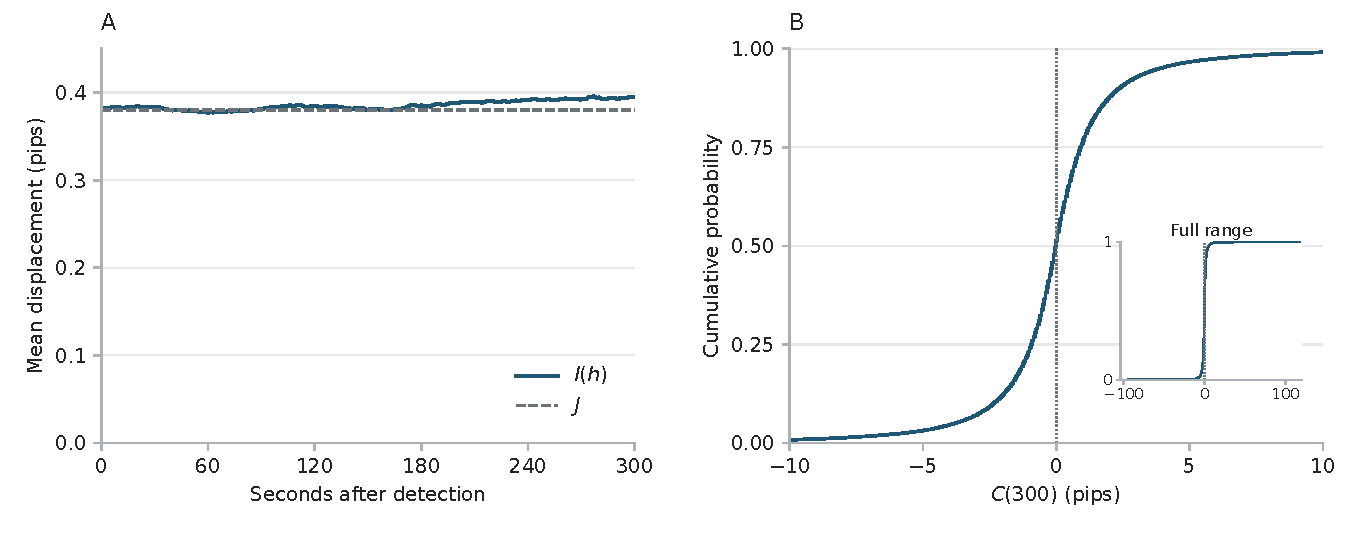
\includegraphics[width=0.96\linewidth]{section4_adjustment.pdf}
\caption{Average displacement and individual subsequent movement. The response path plots mean $I(h)$ from detection through 300 seconds, using the same 127,013 events at every horizon; the dashed line marks mean $J$. The distribution panel plots the empirical cumulative distribution of $C(300)$, or the proportion at or below each value. Its central view covers $-10$ to $10$ pips and its inset retains the full range. All prices use strictly earlier quotes. No uncertainty band is implied.}\label{fig:adjustment}
\end{figure}
\FloatBarrier

The event rule and the initial response share quote observations from the onset second. A positive mean $J$ consequently cannot establish that the detector identifies an exogenous cause of price changes, nor that it predicts those changes before they occur. The decomposition is useful precisely because it prevents movement already used in event recognition from being counted as a subsequent forecast achievement. The observed positive endpoint is an empirical property of these selected events, conditional on the recording and direction conventions.

\subsection{What does the average conceal?}
The right panel of Figure~\ref{fig:adjustment} shows why a nearly unchanged mean is insufficient to describe individual outcomes. The median subsequent movement is zero, but the middle half extends from $-0.95$ to $0.90$ pips and the full-range inset displays the tails omitted by a central view alone. Thus, the small pooled mean coexists with substantial price variation at the event level. Neither the mean nor the median implies that individual prices stop moving at detection.

The orientation also matters. There are 9,267 events with negative initial displacement and 5,442 with zero initial displacement. Keeping them avoids selecting only events whose prices already move with imbalance, and makes a ratio such as $C_i/J_i$ unsuitable as a general persistence measure. A negative subsequent movement means movement against the detected imbalance; it is not automatically a reversal of each event's initial price change. The table and figure retain the underlying pip quantities so these distinctions remain visible.

This distribution motivates the forecasting question. A predictor could distinguish opposing subsequent movements even when they cancel in the average. Conversely, visible dispersion alone does not imply that the chosen history summaries can distinguish them. The next comparisons therefore evaluate actual forecasts of $C(300)$, rather than treating a small mean as evidence for or against predictability.

\subsection{Do the specified additions improve forecasts?}
Neither extension reduces pooled realized error. Table~\ref{tab:forecast} first reports the full forecast rules against the two simple references, then isolates each addition relative to its own benchmark. This ordering separates two questions: whether the fitted procedure performs better than a simple reference, and whether a particular added feature improves that procedure. Success on one comparison would not ensure success on the other.

\begin{table}[htbp]\centering
\caption{Pooled forecast accuracy and incremental differences}\label{tab:forecast}
\begin{tabular}{lrr}\toprule
\multicolumn{3}{l}{Panel A: Forecast rules}\\
Rule & MSE (pips$^2$) & RMSE (pips)\\\midrule
Zero subsequent movement &10.524918&3.244213\\
Matured training mean &10.525069&3.244236\\
Additive benchmark &10.547279&3.247657\\
Additive plus interaction &10.548794&3.247891\\
Richer benchmark &10.584776&3.253425\\
Richer benchmark plus $S$ &10.585063&3.253469\\\midrule
\multicolumn{3}{l}{Panel B: Extension minus its benchmark}\\
Comparison & MSE difference & Relative change (\%)\\\midrule
Pressure--variation &+0.001516&+0.0144\\
Pressure ordering &+0.000287&+0.0027\\\bottomrule
\end{tabular}
\par\smallskip\begin{minipage}{0.94\linewidth}\footnotesize
Every rule predicts $C(300)$ on the same 127,013 outcomes. Positive differences favor the benchmark. Relative changes divide the unrounded difference by the corresponding benchmark MSE. The two pairs have different information sets. RMSE measures forecast-error scale, not average price movement. These are realized losses; no forecast-loss significance tests or intervals are reported.
\end{minipage}\end{table}

The interaction raises MSE by 0.001516 pips squared, or 0.0144\% of the additive benchmark's loss. The corresponding RMSE increase is approximately 0.00023 pips against an error scale near 3.25 pips. Both members of this pair also have greater loss than the zero-movement and matured-mean references. The added interaction therefore supplies no realized gain either by improving its benchmark or by producing the best rule among these reported alternatives.

Adding the ordering statistic raises MSE by 0.000287 pips squared, or 0.0027\% of the richer benchmark's loss, with an RMSE increase of approximately 0.000044 pips. Again, both rules lose to the simple references. The richer benchmark already contains composition and recent pressure and price changes. The finding is therefore about the remaining value of adjacent-sign agreement within that representation, not about whether sequence information is generally irrelevant. Different aggregate statistics, estimators, or populations have not been evaluated by this comparison.

The numerical differences are small, but their smallness does not establish that the rules are equivalent. Nor do their adverse signs establish statistical inferiority: Section~\ref{sec:design} explains why population inference requires more than these historical rankings. For the stated question, the direct answer is that neither specified addition improved the recorded forecasts. This answer retains the unsuccessful comparisons without extending them into a general claim that exchange-rate movement is unpredictable.

\subsection{Are the pooled comparisons uniform across periods?}
Pooling can conceal intervals in which an extension helps, even if its overall difference is adverse. Figure~\ref{fig:quarters} therefore plots extension-minus-benchmark MSE chronologically for every reported quarter. The zero line distinguishes improvement from deterioration, while the pooled diamonds preserve event weighting. The two panels use different benchmarks and should be read as separate incremental comparisons.

\begin{figure}[!ht]\centering
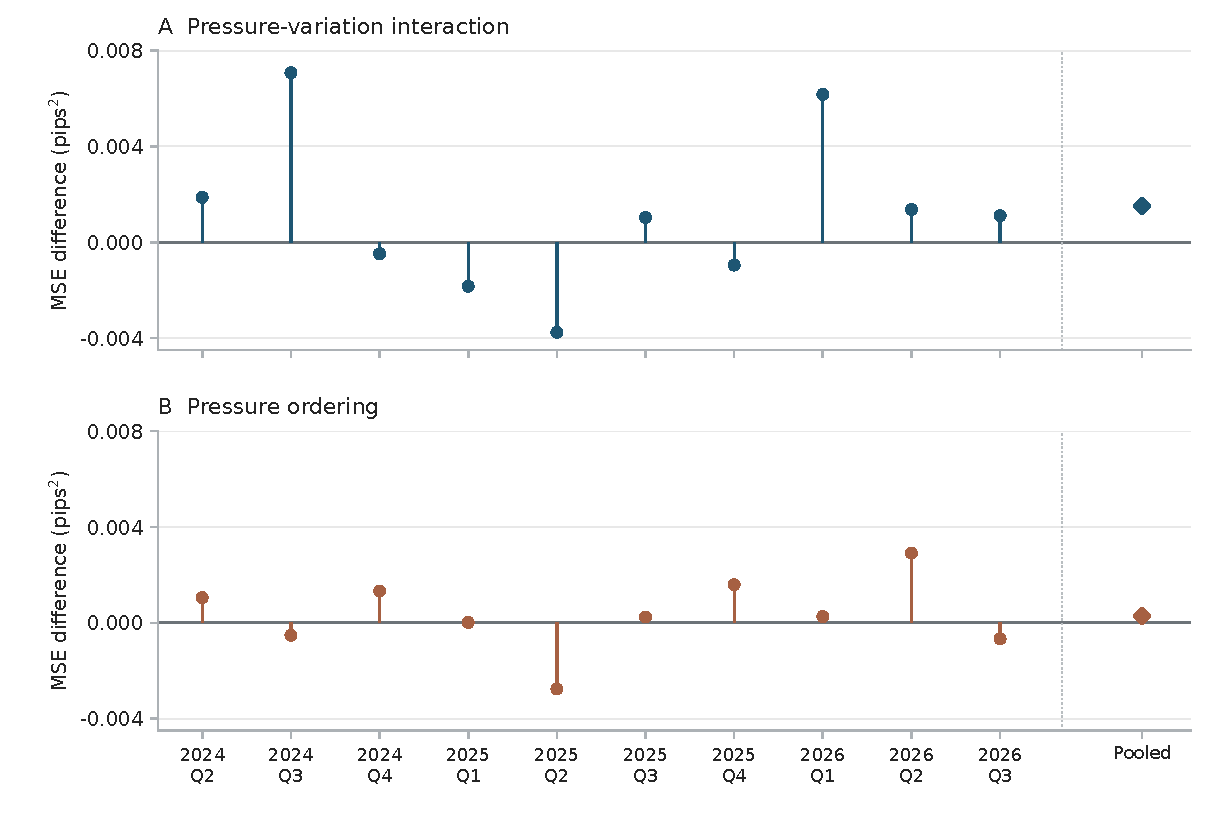
\includegraphics[width=0.96\linewidth]{section4_forecast_quarters.pdf}
\caption{Quarterly incremental forecast differences. Each point is extension-minus-benchmark MSE in pips squared. The interaction is compared with the additive benchmark; the ordering extension is compared with the richer benchmark. Negative values favor the addition. Diamonds give event-weighted pooled differences. All ten periods are retained, including 6 May--June 2024 and July 2026. Stems join estimates to zero and are not uncertainty intervals. Counts and exact values are in Appendix~\ref{app:quarters}.}\label{fig:quarters}
\end{figure}
\FloatBarrier

The interaction improves its benchmark in four quarters and the ordering statistic in three. The pooled adverse signs therefore do not describe every period. However, each of the four regression rules has greater MSE than both simple references in all ten quarters. An incremental improvement within a quarter is consequently distinct from beating the zero or historical-mean rule in that quarter. Calendar decomposition helps reveal this distinction without changing the evaluation population or choosing favorable dates.

These quarters remain subdivisions of one historical record. Counting their signs is neither an independence argument nor a formal stability test. We retain the first and last partial quarters and report their event counts in Appendix~\ref{app:quarters}, so the pooled estimate can be reconstructed rather than mistaken for an equally weighted average of the plotted points. The remaining question concerns the response measurement itself: whether the predominance of initial average displacement depends on the stated horizon and price-age conventions.

\subsection{Measurement restrictions and the separate timing application}
At 60 seconds, mean subsequent movement is $-0.00327$ pips, compared with $0.01475$ pips at 300 seconds on the same events. The interval containing its middle half widens from $[-0.40,0.40]$ to $[-0.95,0.90]$ pips. Additional elapsed time therefore brings greater individual dispersion while average total displacement stays near its initial component. This comparison is descriptive evidence at two finite horizons; it cannot determine the eventual limit of the response.

Requiring more recent prices changes the magnitudes but preserves this ordering of the means. The existing 15-, 30-, and 60-second restrictions require each of the pre-onset, detection, and endpoint quotes to be no older than the cap. Under the strictest cap, 100,248 events remain, with mean initial displacement of 0.40118 pips and mean subsequent movement of 0.02303 pips. Appendix~\ref{app:quoteage} reports all four rows including the baseline. Since these restrictions alter the population, row differences do not isolate a causal effect of quote age. Endpoint age is also future information: these are retrospective measurement checks, not forecast-issuance rules or evidence that forecast rankings survive the same filters.

The duration representation raises a separate question, addressed in Appendix~\ref{app:spread}. Using eligible active seconds rather than event onsets, the supporting application forecasts average quoted spread over the following five minutes. Its benchmark already contains raw and seasonal timing, activity, and quote conditions. Across 19,042,840 paired outcomes, the benchmark reduces MSE by 16.23\% relative to carrying the current spread forward, but adding the duration-normalized summary increases MSE by 0.267\%. A nominal conditional interval for that relative increase is $[-0.080\%,0.614\%]$ and includes zero.

The appendix concentration figure explains where this comparison is determined. The highest training-defined spread category contains 41.8\% of origins and 94.4\% of benchmark squared error. Its deterioration outweighs small improvements in the lower categories. This helps interpret the pooled loss without assigning a mechanism to the pattern. The larger sample and different outcome cannot strengthen the event-price inference; their role is to document another specified application in which the added representation supplies no realized gain.

\FloatBarrier
\section{Conclusion}\label{sec:conclusion}
This study separates displacement already recorded when an unusual quote event becomes detectable from the movement that follows. In the selected EUR/USD sample, mean initial displacement is 0.380 pips and mean displacement five minutes later is 0.395 pips. The difference is small at the level of the average, while individual subsequent movements remain dispersed. An endpoint that retains the initial displacement therefore conveys less about future adjustment than an undivided response measure might suggest.

The forecast comparisons address the conditional question left open by those averages. Adding a pressure--variation interaction does not improve realized accuracy relative to the additive benchmark. Adding adjacent pressure-sign ordering, conditional on composition and richer recent-history controls, likewise does not improve its benchmark. All reported fitted price rules have higher loss than the simple references in every evaluated quarter. These findings concern the specified procedures and history; they do not show that other information or models cannot predict subsequent movement.

The value of the exercise is this explicit connection between measurement time, the outcome remaining to be forecast, and benchmark-relative performance. The price-age and horizon checks retain the predominance of initial average displacement within their respective samples, while the separate spread application documents the limited incremental performance of the timing normalization. Neither exercise identifies the cause of price adjustment or validates the detector as a structural liquidity measure. Generalization would require an independently evaluated sample and a design suited to the stronger claim. Within the present evidence, the defensible conclusion is narrower: retained average displacement coexists with no realized forecasting gain from the specified additions.

\clearpage
\begingroup
\singlespacing\raggedright
\setlength{\bibsep}{6pt}
\begin{thebibliography}{99}
\bibitem[Berger et~al.(2008)]{berger2008order}
Berger, D. W., Chaboud, A. P., Chernenko, S. V., Howorka, E., and Wright, J. H. (2008).
Order flow and exchange rate dynamics in electronic brokerage system data.
\emph{Journal of International Economics}, 75(1), 93--109.
\href{https://doi.org/10.1016/j.jinteco.2007.10.004}{doi:10.1016/j.jinteco.2007.10.004}.

\bibitem[Clark and West(2007)]{clark2007approximately}
Clark, T. E., and West, K. D. (2007).
Approximately normal tests for equal predictive accuracy in nested models.
\emph{Journal of Econometrics}, 138(1), 291--311.
\href{https://doi.org/10.1016/j.jeconom.2006.05.023}{doi:10.1016/j.jeconom.2006.05.023}.

\bibitem[Cont et~al.(2023)]{cont2023cross}
Cont, R., Cucuringu, M., and Zhang, C. (2023).
Cross-impact of order flow imbalance in equity markets.
\emph{Quantitative Finance}, 23(10), 1373--1393.
\href{https://doi.org/10.1080/14697688.2023.2236159}{doi:10.1080/14697688.2023.2236159}.
Accessible author manuscript: \url{https://arxiv.org/abs/2112.13213}.

\bibitem[Cont et~al.(2014)]{cont2014price}
Cont, R., Kukanov, A., and Stoikov, S. (2014).
The price impact of order book events.
\emph{Journal of Financial Econometrics}, 12(1), 47--88.
\href{https://doi.org/10.1093/jjfinec/nbt003}{doi:10.1093/jjfinec/nbt003}.

\bibitem[Dukascopy(2026)]{dukascopyITick}
Dukascopy (2026). \emph{ITick: JForex API documentation}.
\url{https://www.dukascopy.com/client/javadoc3/com/dukascopy/api/ITick.html}.
Accessed 15 October 2026.

\bibitem[Engle and Russell(1997)]{engle1997forecasting}
Engle, R. F., and Russell, J. R. (1997).
Forecasting the frequency of changes in quoted foreign exchange prices with the autoregressive conditional duration model.
\emph{Journal of Empirical Finance}, 4(2--3), 187--212.
\href{https://doi.org/10.1016/S0927-5398(97)00006-6}{doi:10.1016/S0927-5398(97)00006-6}.

\bibitem[Engle and Russell(1998)]{engle1998duration}
Engle, R. F., and Russell, J. R. (1998).
Autoregressive conditional duration: A new model for irregularly spaced transaction data.
\emph{Econometrica}, 66(5), 1127--1162.
\href{https://doi.org/10.2307/2999632}{doi:10.2307/2999632}.

\bibitem[Evans and Lyons(2002)]{evans2002order}
Evans, M. D. D., and Lyons, R. K. (2002).
Order flow and exchange rate dynamics.
\emph{Journal of Political Economy}, 110(1), 170--180.
\href{https://doi.org/10.1086/324391}{doi:10.1086/324391}.

\bibitem[Hashimoto et~al.(2008)]{hashimoto2008random}
Hashimoto, Y., Ito, T., Ohnishi, T., Takayasu, M., Takayasu, H., and Watanabe, T. (2008).
Random walk or a run: Market microstructure analysis of the foreign exchange rate movements based on conditional probability.
NBER Working Paper 14160.
\href{https://doi.org/10.3386/w14160}{doi:10.3386/w14160}.

\bibitem[Ito and Hashimoto(2006)]{ito2006price}
Ito, T., and Hashimoto, Y. (2006).
Price impacts of deals and predictability of the exchange rate movements.
NBER Working Paper 12682.
\href{https://doi.org/10.3386/w12682}{doi:10.3386/w12682}.

\bibitem[Krohn et~al.(2024)]{krohn2024foreign}
Krohn, I., Mueller, P., and Whelan, P. (2024).
Foreign exchange fixings and returns around the clock.
\emph{The Journal of Finance}.
\href{https://doi.org/10.1111/jofi.13306}{doi:10.1111/jofi.13306}.

\bibitem[Newey and West(1994)]{newey1994automatic}
Newey, W. K., and West, K. D. (1994).
Automatic lag selection in covariance matrix estimation.
\emph{The Review of Economic Studies}, 61(4), 631--653.
\href{https://doi.org/10.2307/2297912}{doi:10.2307/2297912}.
\end{thebibliography}

\endgroup
\clearpage
\onehalfspacing
\appendix
\section{Data support, normalization, and detector checks}
\label{app:data}

\subsection{Recorded quotes and observation support}
The archive contains 55,709,907 cached EUR/USD records from January 2024 through July 2026. Removing 1,589 zero-spread records leaves 55,708,318 quotes. The retained observations have finite positive prices, ask above bid, finite nonnegative reported sizes, and strictly increasing timestamps. The nominal weekly calendar follows the New York trading week; 144 nominally open hours have no cached observations. Their causes are unresolved. Weekly closures, absent hours, and intervening removed records divide the retained quotes into 208 structural segments. There are 55,708,110 valid within-segment transitions, while the first observation of each segment has no usable incoming transition.

The baseline permits a previously observed quote to remain the latest quote within structural support without imposing a maximum age. Supported seconds without updates are recorded as zero activity; unsupported seconds remain missing. Complete support is required throughout a measurement window, so available endpoints alone cannot establish availability. These are retrospective conventions for this recorded sample, not a real-time outage detector or a certification of feed completeness.

The bid and ask size fields are quantities reported at the vendor's best quotes. Dukascopy's API describes them as available volumes at those prices, but this does not establish complete market-wide queues. We therefore apply the arithmetic of \citet{cont2014price} as a recorded quote-imbalance measure. Sizes remain in their stored units. The calculation has no spread division or depth normalization. An invalid transition remains unavailable rather than joining nonadjacent quotes, and one unavailable contribution invalidates its second's aggregate. Historical loss of intermediate or size-only updates cannot be ruled out. Consequently, neither the measured imbalance nor its direction identifies executed trading, informed trading, or an exogenous order-flow shock.

\subsection{Historical seasonal factors}
Before UTC day $d$, the absolute-imbalance and update-count factors use eligible seconds in $[d-56\text{ days},d)$. For either channel $x$, the factor is
\begin{equation}
 \phi_{x,d,c}=\frac{\overline{x}_{d,c}}{\overline{x}_{d}},
 \qquad x_s^{\mathrm{adj}}=x_s/\phi_{x,d,c(s)},
 \label{eq:app-seasonal}
\end{equation}
where $c(s)$ denotes its UTC weekday and 15-minute cell. The denominator averages all eligible seconds for that channel in the same historical window; the numerator uses the matching cell. Supported zero-update seconds enter when their measurement is valid. A factor requires a full 56-day history, at least four prior matching dates, and 1,800 eligible seconds. Missing or nonpositive factors remain unavailable without interpolation or cross-cell substitution. UTC cells provide a reproducible convention; they do not perfectly align daylight-saving changes, holidays, or all trading-session patterns.

Duration normalization uses a separate origin-cell calculation. The timescale $g_n$ is observed waiting-time exposure divided by completed waits among historical origins in the matching weekday and 15-minute cell. Exposure includes elapsed portions of unfinished waits and excludes portions after the historical cutoff. In addition to a full 56-day history and four matching dates, the cell requires 1,800 exposure seconds and 100 completions. The assigned $g_n$ stays fixed throughout its wait, including when the wait crosses midnight or a cell boundary.

\subsection{Working duration model and diagnostic limitations}
Following the conditional-duration framework of \citet{engle1998duration}, let $y_n=\Delta_n/g_n$ be a completed, seasonally scaled wait. The retained working model is
\begin{equation}
 y_n=\psi_n\varepsilon_n,\qquad
 \psi_n=\omega+\alpha y_{n-1}+\beta\psi_{n-1},
 \qquad E(\varepsilon_n)=1.
 \label{eq:app-acd}
\end{equation}
For Weibull shape $k$, write $G_k=\Gamma(1+1/k)$. The working conditional cumulative hazard of scaled elapsed time $y$ is
\begin{equation}
 H_n(y)=\left(\frac{G_k y}{\psi_n}\right)^k,
 \qquad
 S_n(y)=\exp[-H_n(y)].
 \label{eq:app-acd-hazard}
\end{equation}
This parameterization gives conditional mean $\psi_n$ for $y_n$. A completed wait contributes its density to the likelihood; positive unfinished exposure contributes survival only. In seconds, the density also includes the factor $1/g_n$. A completion exactly at an estimation cutoff is excluded from that training likelihood and is available in the deployment interval beginning at the cutoff. The likelihood treats the recorded support's stopping mechanism as ignorable for this working calculation; independent censoring by missing or discarded records has not been established.

Every 14 days, the model is fitted to origins in the preceding 56 days, clipping unfinished exposure at the cutoff. The constraints are $\omega>0$, $\alpha,\beta\geq0$, $\alpha+\beta<0.999$, and $0.2\leq k\leq5$. The recurrence resets after a support break, an unavailable factor, or an incomplete preceding wait, with $\psi=\omega/(1-\alpha-\beta)$. Three fixed starts, $(\alpha,\beta,k)=(0.05,0.85,0.7),(0.15,0.70,1),(0.30,0.50,0.5)$, are optimized by L-BFGS-B; the lowest finite objective among successful starts is retained. The intercept starts from the exposure/completion mean multiplied by $1-\alpha-\beta$. The archived implementation records all attempts, transformations, bounds, and convergence criteria. Numerical convergence does not certify a global optimum or distributional adequacy.

At later recalibrations, a wait already in progress retains the seasonal scale, conditional mean, and parameter vintage issued at its origin. New waits use a separate historical refilter under the new parameters. The initial April 22 deployment has a specific initialization convention: its crossing wait is filtered under the initial fit. Those parameters are not claimed to have been available at that earlier wait origin. Calibration residuals are refiltered under the current fitted parameters; deployment completions retain their issued values. Once a wait completes, its detector input uses $r_n=y_n/\psi_n$.

The diagnostics give a substantive reason to retain the word ``working.'' In the initial April 22--May 5 development window, the structural-support Weibull fit has shape 0.743088, $\alpha+\beta=0.998489$, aggregate events-to-hazard ratio 0.996550, and lag-one martingale-residual correlation 0.014381. Nevertheless, its hazard-band screen fails: the first two band ratios are 0 and 0.083687. The screen compares events with integrated hazard exposure, including unfinished spells, rather than applying an uncensored probability-integral-transform test to selected completions. Its declared tolerances are an aggregate ratio in $[0.9,1.1]$, absolute lag-one correlation at most 0.05, and band ratios in $[0.8,1.2]$ where exposure is at least 100. These are descriptive tolerances, not hypothesis-test critical values.

All 58 later fitted cycles also have hazard-band flags; none passes the duration screen. One cycle has a numerical constraint warning, although all fixed optimizer starts report success. The two initial cycles retain their separately archived diagnostics. These failures prevent interpreting normalized waits as a validated probability law or detector distances as shock probabilities. They do not invalidate the deterministic computation of a historical feature, whose usefulness is assessed separately.

\subsection{Detector accounting and existing comparisons}
There are 60 detector calibration/deployment cycles, with a five-day final deployment. On scored calibration seconds, each of the three inputs is centered and divided by its sample standard deviation. Their sample covariance is used without replacing it by a diagonal matrix. The score is evaluated by a Cholesky solve; a singular covariance or condition number above $10^{10}$ stops calculation. The empirical 99th percentile uses linear interpolation, and equality qualifies as an exceedance. A supported quiet second can establish a clear interval without receiving a duration score. Unavailable active seconds interrupt episode continuity. Five consecutive clear seconds close an episode and establish the necessary preceding history for a new confirmed onset. Computational chunks and recalibration dates do not themselves end episodes.

Over the entire April 22, 2024--July 31, 2026 deployment, 20,494,799 eligible seconds produce 213,325 candidate seconds, a realized share of 1.040874\%. There are 135,724 episode fragments, including 13 uncertain beginnings. These are detector-panel counts; the price-forecast sample applies its later evaluation start, direction, history, and outcome restrictions.

An existing separate comparison assesses whether this detector selects larger subsequent quoted spreads than simpler rules. It uses 20,189,813 common eligible active seconds from May 6, 2024 through July 31, 2026 and does not require nonzero imbalance direction. Each rule uses its own historical 99th percentile and the same onset convention. Alternatives include the two-feature Mahalanobis distance, Euclidean distance of the three standardized inputs, their maximum absolute standardized value, individual absolute standardized inputs, current spread, and preceding variation. These rules do not produce equal numbers of events.

The target is mean quoted spread at the following 300 one-second marks. An ordinary-condition reference forecast controls for current and historical spread, variation, activity, quote age, and calendar conditions. Subtracting this forecast supplies an adjusted descriptive comparison; it does not produce a causal effect. The full rule has 133,563 evaluable onsets and mean future spread 0.903578 pips, versus 0.885363 for the two-feature rule. After adjustment, the difference is 0.001827 pips. Table~\ref{tab:detector-check} retains the three primary comparisons.

\begin{table}[htbp]
\centering
\caption{Existing detector comparison: adjusted future spread}
\label{tab:detector-check}
\begin{tabular}{lrr}
\toprule
Benchmark & Full minus benchmark & Nominal 95\% interval\\
\midrule
Imbalance and activity & 0.001827 & $[-0.000861,\ 0.004515]$\\
Diagonal distance & 0.003524 & $[-0.000529,\ 0.007577]$\\
Maximum absolute feature & 0.001261 & $[-0.001907,\ 0.004429]$\\
\bottomrule
\end{tabular}

\smallskip
\begin{minipage}{0.96\linewidth}\footnotesize
Notes: Differences are in pips of mean future spread after subtracting the same past-trained reference. Intervals use daily ratio influences, a 56-day Bartlett covariance, and Bonferroni adjustment across these three comparisons. Their coverage for repeated estimation of the complete pipeline is unvalidated. The 28- and 112-day alternatives also include zero. Event sets and denominators differ across rules.
\end{minipage}
\end{table}

Full and two-feature candidate sets have 93.495\% intersection-to-union overlap. The primary adjusted differences change sign across quarters and become negative under the 15- and 30-second quote-age screens. Those screens also sharply reduce the sample. A fixed spread-decile/hour adjustment gives the same unresolved qualitative result. Exact-onset disagreement groups and supplementary uncertainty calculations remain in the archived comparison; the latter are exploratory because they were computed after viewing primary results. None establishes detector superiority. The reproduction record also retains the eight-benchmark table, calendar results, age restrictions, and secondary 60-second and price-movement diagnostics. This evidence motivates treating the detector as a measurement choice rather than the paper's claimed innovation.
\section{Forecast definitions and reproduction}
\label{app:forecasts}

\subsection{Predictors and fixed scaling}
\label{app:predictors}

All preceding measurements use $[s_i-300,s_i)$, where $s_i$ is the start of the onset second and $t_{0i}=s_i+1$ is detection. Let $u_{ik}=s_i-300+5k$, $k=0,\ldots,60$, and let $Q_{ik}$ be the sum of recorded quote-imbalance contributions in $[u_{i,k-1},u_{ik})$. Supported seconds without updates contribute zero; an invalid observed transition makes the history unavailable. Define
\begin{align}
Q_i&=\sum_{k=1}^{60}Q_{ik}, &
G_i&=\sum_{k=1}^{60}|Q_{ik}|,\\
V_i&=10^4\left\{\sum_{k=1}^{60}
 [\log m(u_{ik}^{-})-\log m(u_{i,k-1}^{-})]^2\right\}^{1/2}.
\end{align}
Here $G_i$ measures absolute pressure across five-second bins; cancellation within a bin remains possible. It is not the sum of absolute quote-level contributions. $V_i$ is expressed in basis points of log return, whereas the displacement variables $J_i$, $C_i$, and $I_i$ are in pips of the exchange-rate level.

The reference sample comprises 1,281,932 detector-eligible calibration seconds from 26 February through 21 April 2024 with available $Q_i$ and $V_i$. Another 184 calibration seconds lack these states. Selection does not use event membership or future returns. With population denominators, $c_Q=\sqrt{\operatorname{mean}(Q^2)}$, $c_V=\operatorname{mean}(V)$, and $s_V=\sqrt{\operatorname{mean}[(V-c_V)^2]}$. Their frozen values are
\[
 c_Q=134.54108927243408,\qquad
 c_V=1.962402411840539,\qquad
 s_V=1.5415551698605312.
\]
Write $P_i=Q_i/c_Q$, $M_i=|Q_i|/c_Q$, and $v_i=(V_i-c_V)/s_V$. Pressure is not mean-centered, so zero retains its meaning. These constants set units; they are not re-estimated from evaluation outcomes.

Let $B_i=10^4[a(s_i^-)-b(s_i^-)]$ be the preceding spread, $L_i=\log[q^a(s_i^-)+q^b(s_i^-)]$ the log of the positive total vendor-reported size, and $N_i$ the number of preceding quote updates. For $h\in\{5,30\}$, define
\[
 Q_{i,h}=\sum_{k=61-h/5}^{60}Q_{ik},\qquad
 G_{i,h}=\sum_{k=61-h/5}^{60}|Q_{ik}|.
\]
The direction-aligned preceding price change is
\[
 R_{i,h}=10^4d_i[m(s_i^-)-m((s_i-h)^-)],
 \qquad h\in\{5,30,300\}.
\]
All price marks are the last admissible quote strictly before the indicated boundary, within the same observation-support segment.

For the sequence measurement, $z_{ik}=\operatorname{sign}(Q_{ik})$ retains zero bins. Set
\[
 A_i=\frac{1}{59}\sum_{k=1}^{59}z_{ik}z_{i,k+1},\qquad
 A_i^{\mathrm{comp}}=
 \frac{(\sum_{k=1}^{60}z_{ik})^2-\sum_{k=1}^{60}z_{ik}^2}{60\cdot59},
 \qquad S_i=A_i-A_i^{\mathrm{comp}}.
\]
$A_i^{\mathrm{comp}}$ is the exact mean adjacent product under random rearrangement of that observation's fixed signs. This algebraic reference does not assume that market observations are exchangeable or supply a permutation test. A sequence of exclusively positive signs has $S_i=0$, as does an exclusively negative sequence: all its adjacent agreement is already implied by composition. Hence zero $S_i$ cannot be interpreted as absent pressure.

The additive forecast contains an intercept, $(P_i,M_i,v_i,B_i,L_i)$, and the calendar indicators below. Its extension adds only $M_iv_i$. The richer benchmark contains an intercept and the following 19 numeric columns, in addition to the same calendar indicators:
\begin{align*}
(&d_i,J_i,d_iP_i,M_i,G_i/c_Q,v_i,B_i,L_i,\log(1+N_i),\\
 &d_i\textstyle\sum_k z_{ik}/60,\ \textstyle\sum_k z_{ik}^2/60,\ A_i^{\mathrm{comp}},\\
 &d_iQ_{i,5}/c_Q,\ d_iQ_{i,30}/c_Q,\ G_{i,5}/c_Q,\ G_{i,30}/c_Q,\\
 &R_{i,5},R_{i,30},R_{i,300}).
\end{align*}
Its extension adds only $S_i$. Because $A_i^{\mathrm{comp}}$ is already a benchmark column, adding $S_i$ spans the same linear predictor space as adding $A_i$. Recent pressure and price changes also contain ordering information. The comparison therefore concerns this additional adjacent-product representation conditional on the specified benchmark; it does not compare a history-free model with all possible sequence information.

\subsection{Fitting and forecast issuance}
\label{app:fitting}

The 59 fit cutoffs occur every 14 days from 6 May 2024 through 27 July 2026. At cutoff $T$, the expanding training sample contains eligible earlier origins with available five-minute labels satisfying $t_{0i}+300\leq T$. This condition uses the target boundary, even when the quote carried to that boundary is older. The first fit contains 1,782 matured outcomes; the last contains 127,523, including the initial training period before evaluation. Each fit is deployed over $[T,T+14\text{ days})$, with the last interval ending on 1 August 2026. The mean reference uses precisely the same matured training outcomes; the zero reference requires no fit.

Hour indicators use 00 UTC as reference and include 01--23; weekday indicators use Monday as reference and include Tuesday--Friday and Sunday. Saturday is outside the inherited supported calendar. Within a training sample, an identically zero calendar indicator is omitted and its absent level recorded. If an origin's hour or weekday has not previously occurred in training, both fitted rules in that comparison issue the same training-mean forecast. Two origins receive this fallback in each comparison; they remain in the loss denominator and contribute zero to the paired extension-minus-benchmark difference. An unseen combination of individually observed hour and weekday levels does not trigger the fallback.

Each regression is unpenalized ordinary least squares. For numerical conditioning only, each design column is divided by its root mean square in the training sample; coefficients are mapped back after singular-value decomposition. The design must have more rows than active columns and full numerical rank at tolerance $\epsilon\max(n,p)\sigma_{\max}$ for the equilibrated matrix. Scientific predictors are not dropped, outcomes are not trimmed, and forecasts are not clipped. An independent implementation reconstructs the fits by QR decomposition. The largest equilibrated condition numbers are 19.57 and 76.75 for the interaction and sequence comparisons, respectively.

Each comparison therefore entails 118 regression fits and 59 mean calibrations, not 118 alternative specifications. All 127,058 eligible evaluation origins receive each forecast before future labels are joined. The 45 subsequently unavailable labels leave 127,013 common scored observations. Outcome availability restricts evaluation, not issuance. Forecasts assume zero processing latency; the replay does not establish a practically executable trading rule.

\subsection{Reproducing the reported evidence}
\label{app:reproduction}

The archived prediction ledger separates origins, predictors, labels, fit windows, and window membership. For each comparison, the saved forecast table is created and hashed before its evaluation table. Reproduction proceeds by checking source hashes and origin identities; reconstructing only matured training samples and permitted predictors; checking fitted coefficients and saved forecasts; and then joining outcomes to reconstruct event errors, daily sums, quarterly sums, and pooled accuracy. Pooled MSE is total squared error divided by total scored events, not an equally weighted average of daily or quarterly MSEs. The stable paired-loss identity
\[
 (y_i-f_i)^2-(y_i-b_i)^2=(b_i-f_i)(2y_i-f_i-b_i)
\]
is checked against direct squared losses. Here $b_i$ and $f_i$ are the benchmark and extension forecasts. Both forms use identical observations.

The reproduction archive identifies the source tables as \path{step09a_prediction_ledger_20261003}, \path{step09b_persistence_forecast_20261003}, and \path{step10b_sequence_forecast_20261003} under \texttt{data/signals}. Each contains its manifest and verification results; the forecast runs also preserve the executed source and tests. The response membership and uncertainty archives are \path{step07m_joint_response_20261002} and \path{step07n_joint_uncertainty_20261002}. These identifiers distinguish the reported calculation from superseded exploratory outputs. Revising the paper recomputes reporting summaries from these saved records, without fitting further models.

\section{Uncertainty, calendar comparisons, and measurement restrictions}
\label{app:checks}

\subsection{Uncertainty around mean displacement}
\label{app:uncertainty}

For component $x_i\in\{J_i,C_i(h),I_i(h)\}$ and a declared cohort, let $N$ be its event count and $\bar x=N^{-1}\sum_i x_i$. On UTC onset date $t$, with $n_t$ selected events, define the daily influence
\[
 u_t=N^{-1}\left(\sum_{i\in t}x_i-n_t\bar x\right).
\]
All 817 calendar dates from 6 May 2024 through 31 July 2026 are retained, including zero-event dates. Those dates have zero observed scores; they do not represent imputed price changes or verified feed completeness. Stack the influences for $J,C,I$ at 60 and 300 seconds, both on each horizon's available cohort and on their common cohort, into the 12-vector $\mathbf u_t$. The reported covariance is
\begin{align}
 \widehat\Omega_L={}&\sum_{t=1}^{817}\mathbf u_t\mathbf u_t'
 +\sum_{\ell=1}^{L}\left(1-\frac{\ell}{L+1}\right)
 \sum_{t=\ell+1}^{817}
 (\mathbf u_t\mathbf u_{t-\ell}'+\mathbf u_{t-\ell}\mathbf u_t').
\end{align}
This calendar aggregation allows cross-event dependence within dates and serial covariance across dates. There is no prewhitening or degrees-of-freedom correction. The identity $I=J+C$, and repeated observations across the two cohorts, make the joint covariance singular by construction; no inverse is required for marginal intervals.

The scalar Bartlett bandwidth calculation follows \citet{newey1994automatic}. For each coordinate, use pilot lag $m=\lfloor4(817/100)^{2/9}\rfloor$, pilot autocovariances $\gamma_j=817^{-1}\sum_{t=j+1}^{817}u_tu_{t-j}$, $s_0=\gamma_0+2\sum_{j=1}^{m}\gamma_j$, and $s_1=2\sum_{j=1}^{m}j\gamma_j$. The continuous bandwidth is $1.1447[817(s_1/s_0)^2]^{1/3}$. Taking the floor of the largest bandwidth across the 12 coordinates gives the common lag $L=20$; the declared longer calculation uses $2L=40$. This coordinate-maximum rule is a project choice, not a claim of multivariate optimality or guaranteed conservative coverage.

Table~\ref{tab:lagchecks} reports $\bar x\pm z_{0.975}\sqrt{\widehat\Omega_{L,xx}}$, where $z_{0.975}$ is the standard-normal 97.5th percentile. They are pointwise nominal intervals for a hypothetical repeated selected-event process under suitable stability, moment, dependence, and normal-approximation conditions. Those conditions and full adaptive-pipeline coverage have not been established. The intervals are neither simultaneous bands for the response path nor tests that the small mean continuation is economically equivalent to zero.

\begin{table}[htbp]
\centering
\caption{Displacement means and nominal lag sensitivity}
\label{tab:lagchecks}
\small\setlength{\tabcolsep}{3pt}
\begin{tabular}{llrrr}
\toprule
Cohort and horizon & Component & Mean & 20-day interval & 40-day interval\\
\midrule
Common, 60 seconds & $J$ & 0.380258 & [0.341466, 0.419049] & [0.332622, 0.427893]\\
 & $C(60)$ & -0.003271 & [-0.013836, 0.007294] & [-0.013404, 0.006862]\\
 & $I(60)$ & 0.376987 & [0.339522, 0.414451] & [0.330708, 0.423265]\\
Common, 300 seconds & $J$ & 0.380258 & [0.341466, 0.419049] & [0.332622, 0.427893]\\
 & $C(300)$ & 0.014752 & [-0.004937, 0.034442] & [-0.004179, 0.033684]\\
 & $I(300)$ & 0.395010 & [0.347638, 0.442381] & [0.337562, 0.452457]\\
Available, 60 seconds & $J$ & 0.380295 & [0.341517, 0.419074] & [0.332673, 0.427918]\\
 & $C(60)$ & -0.003153 & [-0.013754, 0.007448] & [-0.013329, 0.007023]\\
 & $I(60)$ & 0.377142 & [0.339739, 0.414546] & [0.330936, 0.423348]\\
\bottomrule
\end{tabular}
\begin{minipage}{0.98\linewidth}\small
\emph{Notes:} All entries are pips. The common cohort has 127,013 events. The separately available 60-second cohort has 127,052, including 39 events without a five-minute endpoint. The available five-minute cohort is identical to the common cohort. Intervals use the full joint covariance described in the text; longer lags need not widen them.
\end{minipage}
\end{table}

Concentration remains relevant even with daily aggregation. For the primary five-minute means, the largest daily squared-influence shares are 9.63\% for $J$ (9 April 2025), 24.56\% for $C$ (2 April 2025), and 22.86\% for $I$ (2 April 2025). These shares divide a day's squared influence by the sum of squared daily influences, not by the full Bartlett variance. They neither count independent dates nor justify deleting influential observations.

\subsection{Complete calendar comparisons}
\label{app:quarters}

Table~\ref{tab:fullquarters} reports every evaluation quarter, including the initial and final partial quarters. Negative differences favor the extension. Their pooled counterparts weight events: for quarterly event counts $N_q$ and mean differences $\bar\delta_q$, the pooled difference is $\sum_qN_q\bar\delta_q/\sum_qN_q$. This explains why the number of favorable quarters cannot substitute for the pooled comparison. All four fitted rules have higher realized MSE than the zero and training-mean references in every reported quarter.

\begin{table}[htbp]
\centering
\caption{Complete quarterly price-forecast accuracy}
\label{tab:fullquarters}
\small
\setlength{\tabcolsep}{3pt}
\begin{tabular}{lrrrrrrr}
\toprule
Quarter & Events & Zero & Mean & Additive & Rich & $\Delta_{\rm int}$ & $\Delta_{\rm seq}$\\
\midrule
2024 Q2$^{a}$ & 7,116 & 1.177593 & 1.178304 & 1.254800 & 1.332271 & +0.001870 & +0.001054 \\
2024 Q3 & 17,227 & 2.387362 & 2.387636 & 2.392969 & 2.396611 & +0.007069 & -0.000519 \\
2024 Q4 & 17,148 & 10.775509 & 10.776085 & 10.801820 & 10.831613 & -0.000478 & +0.001330 \\
2025 Q1 & 11,280 & 12.642316 & 12.642345 & 12.644223 & 12.705992 & -0.001837 & +0.000018 \\
2025 Q2 & 14,363 & 32.690695 & 32.691484 & 32.768045 & 32.927081 & -0.003761 & -0.002756 \\
2025 Q3 & 13,904 & 6.819343 & 6.819425 & 6.838044 & 6.821225 & +0.001026 & +0.000248 \\
2025 Q4 & 10,883 & 3.480357 & 3.481135 & 3.489368 & 3.490698 & -0.000955 & +0.001595 \\
2026 Q1 & 18,729 & 14.976527 & 14.975046 & 14.986956 & 15.024415 & +0.006164 & +0.000266 \\
2026 Q2 & 11,081 & 5.824517 & 5.825187 & 5.826771 & 5.844462 & +0.001368 & +0.002909 \\
2026 Q3$^{b}$ & 5,282 & 2.393913 & 2.393632 & 2.399976 & 2.395902 & +0.001111 & -0.000663 \\
\bottomrule
\end{tabular}
\begin{minipage}{0.98\linewidth}\small
\emph{Notes:} MSE and differences are in pips squared. $\Delta_{\rm int}$ is interaction minus additive; $\Delta_{\rm seq}$ is sequence extension minus rich benchmark. Thus each extension's MSE equals its benchmark MSE plus the displayed difference, subject to rounding. $^{a}$6 May--30 June 2024. $^{b}$July 2026 only. Every column uses the same events within a quarter. Neither these realized differences nor their signs establish population forecast superiority.
\end{minipage}
\end{table}

For the two primary contrasts, let $D_t=\sum_{i\in t}\delta_i$ and $\psi_t=D_t-n_t\bar\delta$, grouped by UTC forecast-origin date, with all 817 dates retained; 701 contain scored origins. The largest $|D_t|/\sum_s|D_s|$ is 10.77\% for the interaction comparison (2 April 2025) and 3.46\% for the sequence comparison (11 April 2025). The corresponding maximum $\psi_t^2/\sum_s\psi_s^2$ shares are 38.99\% and 19.19\%. Saved cross-products through lag 40 describe temporal dependence. These concentration and serial diagnostics do not establish the null distribution of a nested forecast comparison. Estimating extra coefficients can itself raise realized error even under equal population predictive content \citep{clark2007approximately}; no conventional price-forecast significance test is inferred from the descriptive differences.

\subsection{Quote-age restrictions}
\label{app:quoteage}

Let a mark's age be its requested boundary minus the timestamp of its strictly earlier source quote. Table~\ref{tab:quoteage} restricts the three marks defining $J_i$ and $C_i(300)$---before onset, at detection, and at the five-minute endpoint---to ages no greater than the indicated cap. The inequalities are inclusive. These checks do not constrain every intermediate quote in the path, and the endpoint restriction is known only retrospectively.

\begin{table}[htbp]
\centering
\caption{Five-minute response means under three-mark quote-age restrictions}
\label{tab:quoteage}
\begin{tabular}{lrrrr}
\toprule
Maximum age & Events & $\bar J$ & $\bar C(300)$ & $\bar I(300)$\\
\midrule
No additional cap & 127,013 & 0.380258 & 0.014752 & 0.395010\\
15 seconds & 100,248 & 0.401176 & 0.023034 & 0.424210\\
30 seconds & 116,836 & 0.388115 & 0.018143 & 0.406257\\
60 seconds & 125,127 & 0.381103 & 0.016353 & 0.397456\\
\bottomrule
\end{tabular}
\begin{minipage}{0.98\linewidth}\small
\emph{Notes:} Means are in pips and satisfy $\bar I=\bar J+\bar C$ before rounding. Each restricted row is a subset of the same 127,013-event five-minute cohort. These are descriptive re-aggregations, with no newly estimated interval or forecast model.
\end{minipage}
\end{table}

The initial component remains much larger than average subsequent movement under each restriction. Because the retained populations differ, these comparisons combine measurement freshness and sample composition; they are not controlled estimates of stale-quote bias. They also do not establish that forecast rankings survive the restrictions. Similarly, sampling-grid checks performed for earlier conditional-association regressions are not represented as robustness checks for the current forecast equations.
\section{A separate forecast of subsequent quoted spreads}
\label{app:spread}

\subsection{Question, population and timing}

The supporting exercise asks whether dynamic duration normalization adds predictive value after raw and seasonally adjusted timing, quote ages, activity and other observed quote conditions have already entered a benchmark. Its outcome and population differ from the event-price comparisons. Let $w(u^-)=10^4[a(u^-)-b(u^-)]$ denote the strict-left quoted spread in pips. For an eligible active second $[s,s+1)$, the forecast is issued at $t_0=s+1$ and predicts
\begin{equation}
 Y_s=\frac{1}{300}\sum_{j=1}^{300}w((t_0+j)^-).
 \label{eq:spread-target}
\end{equation}
All marks must remain within the archived structural support. The target is a mean recorded quoted spread; it does not measure executed trading costs, available depth or execution probability. Neither detector exceedance nor event direction selects this population.

The predictor and outcome archives begin on 6 May 2024. Requiring a full 56-day training history moves the first evaluation cutoff to 1 July 2024. Evaluation ends on 31 July 2026. Of 19,065,217 scored origins, 5,336 lack complete predictors and 19,059,881 receive forecasts. A further 17,041 issued forecasts have no available future label, leaving 19,042,840 paired outcomes. Forecasts are generated before future labels are attached and are retained when those labels are unavailable. The evaluation therefore conditions on subsequently evaluable outcomes without using their availability to decide whether to issue a forecast. Zero-update intervals are outside this active-second population.

\subsection{Fixed model pair and training rules}

Both rules use the same histogram gradient-boosted regression procedure and training rows. At each of 55 fortnightly cutoffs $c$, eligible training bins satisfy $s\geq c-56$ days and $s+301\text{ seconds}\leq c$. The second restriction requires the complete outcome horizon to have elapsed. Complete predictors and available finite labels are also required. A fixed SplitMix64 hash of the origin's integer UTC second, retained when its remainder modulo 20 is zero, provides an approximately 5\% training sample independent of outcomes. This yields 3,837,748 training-origin instances across the overlapping windows; repeated use of an origin is not a new observation. The fit requires at least 1,000 rows.

Table~\ref{tab:spread-features} defines the 16 benchmark inputs. Write $a_q(u)$ for the age in seconds of the quote used at the strict-left boundary $u$, and let $\mathcal{U}_s$ be the completed incoming interquote durations whose endpoints lie in $[s,s+1)$. The raw and seasonal timing summaries are
\begin{equation}
 R_s=-\log\!\left(\frac{1}{N_s}\sum_{n\in\mathcal{U}_s}\Delta_n\right),
 \qquad
 G_s=-\log\!\left(\frac{1}{N_s}\sum_{n\in\mathcal{U}_s}\frac{\Delta_n}{g_n}\right).
 \label{eq:spread-raw-seasonal}
\end{equation}
The seasonal scale $g_n$ is the scale issued at that duration's origin. The raw mean obeys the verified identity $\overline\Delta_s=[1+a_q(s)-a_q(t_0)]/N_s$. Including its logarithm explicitly gives the finite learner this transformation even though the ages and count already determine it algebraically.

\begin{table}[tbp]
\centering\small
\caption{Benchmark inputs in the separate spread forecast}
\label{tab:spread-features}
\begin{tabular}{p{0.29\linewidth}p{0.64\linewidth}}
\toprule
Input & Definition available at $t_0=s+1$ \\
\midrule
Current and pre-bin spreads & $w(t_0^-)$ and $w(s^-)$, in pips. \\
Historical spread & Mean of $w(u^-)$ at the 300 integer-second boundaries $u=s-299,\ldots,s$, in pips. \\
Pre-bin variation & The square root of the sum of the 60 five-second squared log returns ending at $s$, multiplied by $10^4$; basis points. \\
Current activity & $\log(1+N_s)$. \\
Historical activity & $\log(1+\overline N_s)$, where $\overline N_s$ is mean per-second update count over $[s-300,s)$. \\
Current and historical quote ages & $a_q(t_0)$ and the maximum age over the 300 boundaries $s-299,\ldots,s$, in seconds. \\
Calendar & Integer UTC hour and weekday of $s$. \\
Quote imbalance and adjusted activity & Signed $E_s$, seasonally adjusted $|E_s|$, and seasonally adjusted $N_s$. \\
Pre-bin quote age & $a_q(s)$, in seconds. \\
Raw and seasonal timing & $R_s$ and $G_s$ in Equation~\eqref{eq:spread-raw-seasonal}. \\
\bottomrule
\end{tabular}
\end{table}

The extension adds only $T_s=-\log(N_s^{-1}\sum_{n\in\mathcal{U}_s}r_n)$, the working ACD-normalized timing summary used in event measurement. Averaging precedes the logarithm in all three timing summaries. The originally issued duration states are retained; this comparison does not re-estimate the ACD model or refilter past predictors using later parameter estimates. Consequently, the extension changes the representation of recorded history. Its comparison cannot isolate the causal effect of arrivals, or a state known entirely before the current bin: the effective normalization also depends on the completed within-bin durations.

Both fits use squared-error loss, learning rate 0.05, 100 boosting iterations, at most 15 leaves, at least 100 observations per leaf, $L_2$ regularization 1, 63 histogram bins, no early stopping, and random seed 20261004. The specification was fixed before this pair was fitted, after earlier analysis of the same cache. There was no tuning search within the comparison. It remains an exploratory historical evaluation rather than an untouched confirmation sample. Carrying $w(t_0^-)$ forward is retained as an unfitted diagnostic reference.

\subsection{Accuracy, conditional uncertainty and concentration}

\begin{table}[tbp]
\centering\small
\caption{Accuracy of five-minute average-spread forecasts}
\label{tab:spread-accuracy}
\begin{tabular}{lrr}
\toprule
Forecast & MSE (pips$^2$) & RMSE (pips) \\
\midrule
Current-spread carry & 0.051268467 & 0.226425411 \\
Timing and quote-condition benchmark & 0.042948734 & 0.207240763 \\
Benchmark plus ACD-normalized timing & 0.043063423 & 0.207517283 \\
\bottomrule
\end{tabular}
\end{table}

Adding normalized timing increases realized MSE by 0.000114689 pips$^2$, or 0.267037\% of benchmark MSE; RMSE rises by about 0.000277 pips. The whole benchmark procedure improves MSE by 16.23\% relative to carrying the current spread forward, but that comparison does not attribute its gain to any individual feature.

For uncertainty, let $D_d$ be the sum of extension-minus-benchmark squared losses on UTC date $d$, $B_d$ the sum of benchmark squared losses, and $n_d$ the number of paired outcomes. Set $N=\sum_dn_d$, $B=\sum_d B_d$, $\widehat\Delta=\sum_d D_d/N$, and $\widehat\rho=\sum_dD_d/B$. Daily influences are
\begin{equation}
 u_d=\frac{D_d-\widehat\Delta n_d}{N},\qquad
 v_d=\frac{D_d-\widehat\rho B_d}{B}.
\end{equation}
For either influence series $x_d$, the estimated variance is
\begin{equation}
 \widehat V_L(x)=\sum_dx_d^2+
 2\sum_{\ell=1}^{L}\left(1-\frac{\ell}{L+1}\right)
 \sum_{d=\ell+1}^{761}x_dx_{d-\ell}.
\end{equation}
The 761-day calendar retains zero-observation dates. The declared primary lag is 56 calendar days; 28 and 112 days are sensitivity choices. Normal intervals use approximately 1.96 standard errors. Using $v_d$ accounts for estimation of the benchmark-loss denominator rather than dividing a difference interval by that denominator. The primary nominal 95\% interval for the MSE increase is $[-0.000049315,0.000278693]$ pips$^2$.

\begin{table}[tbp]
\centering\small
\caption{Nominal conditional intervals for relative MSE increase}
\label{tab:spread-intervals}
\begin{tabular}{lr}
\toprule
Calendar-day lag & 95\% interval (\%) \\
\midrule
56 (primary) & $[-0.080,\;0.614]$ \\
28 & $[-0.081,\;0.616]$ \\
112 & $[-0.074,\;0.608]$ \\
\bottomrule
\end{tabular}
\end{table}

Every interval includes zero. These calculations condition on the issued forecasts; they do not establish repeated-estimation coverage for the complete rolling pipeline. The overlapping outcomes are not independent replications. No operational materiality margin was justified, so these bounds establish neither equivalence nor economic negligibility.

The pooled increase can conceal both gains and losses across observations. Figure~\ref{fig:spread-concentration} therefore compares each spread category's share of origins with its share of benchmark squared error, then places its incremental forecast difference alongside that concentration. Categories are defined using the current-spread quartiles in each cycle's actual training sample. Values equal to a cutoff enter the higher category; ties are retained. Thus the groups need not each contain 25\% of evaluation origins, and a pooled category does not denote a single absolute spread range.

\begin{figure}[tbp]
\centering
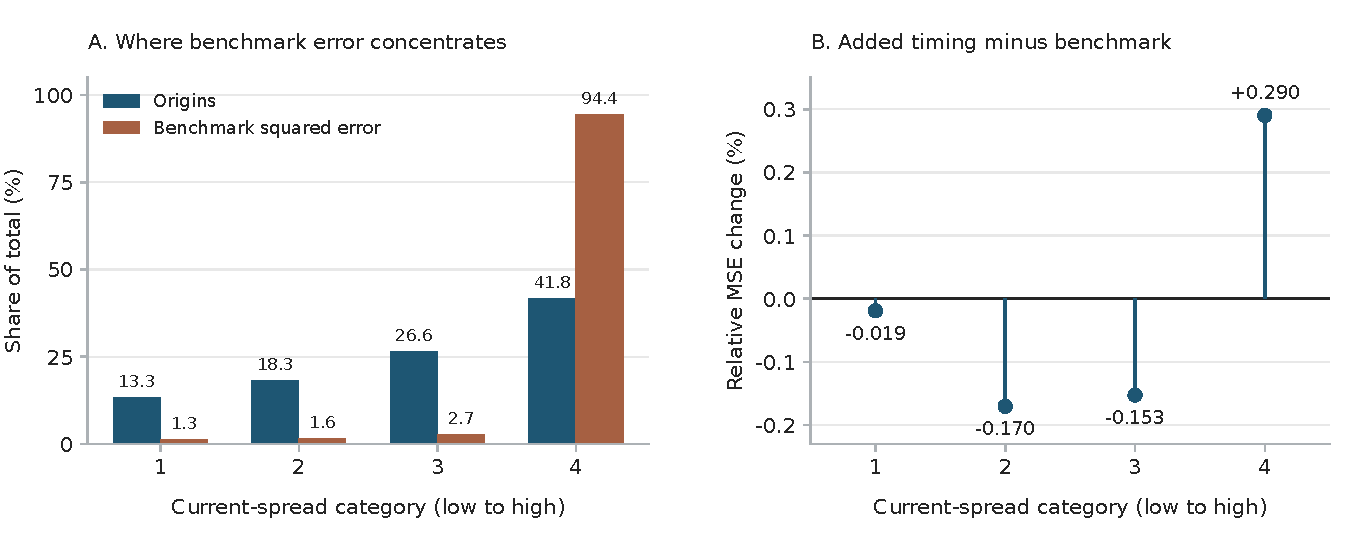
\includegraphics[width=\linewidth]{appendix_spread_concentration.pdf}
\caption{Where the separate spread-forecast comparison is determined. The same 19,042,840 paired outcomes enter both panels. Panel A compares shares of origins and benchmark total squared error. Panel B reports $100(\mathrm{MSE}_{T,g}/\mathrm{MSE}_{B,g}-1)$ within each training-defined current-spread category; negative values favor added timing. Stems connect descriptive estimates to zero and are not uncertainty intervals. Categories retain ties and all observations.}
\label{fig:spread-concentration}
\end{figure}

The highest category contains 41.8\% of origins and 94.4\% of benchmark squared error. The extension slightly improves all three lower-category point estimates, with a combined summed loss reduction of 57.97 pips$^2$, while increasing loss in the highest category by 2,241.97 pips$^2$. This arithmetic explains why the pooled comparison is adverse. It does not show that wider spreads cause the extension to fail: squared loss can concentrate in difficult observations, and these groups also differ in other conditions.

\subsection{Complete declared descriptive checks}

Table~\ref{tab:spread-patterns} retains all specified spread, timing, activity, UTC-block and calendar-quarter comparisons. Timing categories use prior-training quartiles of $T_s$ under the same tie convention. No subgroup inference is performed. All four UTC blocks, all three update-count groups and all four timing categories have adverse point estimates, while three of nine quarters favor the extension. The 18:00--23:59 UTC block contains 15.8\% of origins and 88.3\% of benchmark squared error. Such a broad time block does not identify a rollover, closure or fixing mechanism. The saved per-cycle coverage table preserves all 825 planned non-quarter cells, including 16 with no evaluated outcomes.

{\footnotesize\setlength{\tabcolsep}{3pt}
\begin{longtable}{lrrrrrrr}
\caption{All declared spread-forecast diagnostics}\label{tab:spread-patterns}\\
\toprule
Category & $N$ & Mean $Y$ & Mean $\widehat Y_B$ & Mean $\widehat Y_T$ & MSE$_B$ & MSE$_T$ & Change (\%) \\
\midrule
\endfirsthead
\multicolumn{8}{l}{\textit{Table \thetable\ continued}}\\
\toprule
Category & $N$ & Mean $Y$ & Mean $\widehat Y_B$ & Mean $\widehat Y_T$ & MSE$_B$ & MSE$_T$ & Change (\%) \\
\midrule
\endhead
\bottomrule
\endfoot
\multicolumn{8}{l}{\textit{Current-spread category}}\\
1 & 2,538,115 & 0.3263 & 0.3393 & 0.3393 & 0.004212 & 0.004211 & -0.019 \\
2 & 3,486,743 & 0.3659 & 0.3710 & 0.3710 & 0.003701 & 0.003694 & -0.170 \\
3 & 5,060,569 & 0.3389 & 0.3391 & 0.3391 & 0.004395 & 0.004389 & -0.153 \\
4 & 7,957,413 & 0.5025 & 0.4950 & 0.4950 & 0.097020 & 0.097302 & +0.290 \\
\addlinespace
\multicolumn{8}{l}{\textit{UTC hour block}}\\
00--05 & 3,738,088 & 0.4093 & 0.4044 & 0.4047 & 0.008541 & 0.008604 & +0.739 \\
06--11 & 5,548,160 & 0.3552 & 0.3569 & 0.3569 & 0.007009 & 0.007072 & +0.898 \\
12--17 & 6,747,027 & 0.3419 & 0.3458 & 0.3457 & 0.003648 & 0.003711 & +1.725 \\
18--23 & 3,009,565 & 0.6679 & 0.6596 & 0.6594 & 0.240047 & 0.240437 & +0.163 \\
\addlinespace
\multicolumn{8}{l}{\textit{Updates in the current second}}\\
1 & 7,416,749 & 0.4166 & 0.4170 & 0.4169 & 0.053884 & 0.053977 & +0.173 \\
2--4 & 9,436,148 & 0.3987 & 0.3989 & 0.3989 & 0.033429 & 0.033561 & +0.395 \\
5+ & 2,189,943 & 0.4410 & 0.4354 & 0.4355 & 0.046935 & 0.047048 & +0.242 \\
\addlinespace
\multicolumn{8}{l}{\textit{Normalized-timing category}}\\
1 & 4,775,025 & 0.4027 & 0.4034 & 0.4032 & 0.037441 & 0.037585 & +0.385 \\
2 & 4,788,010 & 0.3978 & 0.3974 & 0.3973 & 0.031287 & 0.031359 & +0.228 \\
3 & 4,763,161 & 0.4048 & 0.4036 & 0.4036 & 0.037171 & 0.037287 & +0.313 \\
4 & 4,716,644 & 0.4371 & 0.4365 & 0.4367 & 0.066197 & 0.066324 & +0.192 \\
\addlinespace
\multicolumn{8}{l}{\textit{Calendar quarter}}\\
2024Q3 & 2,219,772 & 0.2512 & 0.2462 & 0.2462 & 0.012172 & 0.012142 & -0.246 \\
2024Q4 & 2,402,729 & 0.2892 & 0.2817 & 0.2817 & 0.040518 & 0.040523 & +0.013 \\
2025Q1 & 2,562,104 & 0.4843 & 0.4718 & 0.4717 & 0.034852 & 0.034765 & -0.249 \\
2025Q2 & 2,960,452 & 0.6083 & 0.6163 & 0.6165 & 0.062028 & 0.062563 & +0.861 \\
2025Q3 & 1,998,986 & 0.4516 & 0.4630 & 0.4630 & 0.041477 & 0.041541 & +0.154 \\
2025Q4 & 1,867,692 & 0.4308 & 0.4253 & 0.4252 & 0.060409 & 0.060326 & -0.137 \\
2026Q1 & 2,237,819 & 0.3569 & 0.3639 & 0.3637 & 0.030444 & 0.030467 & +0.074 \\
2026Q2 & 2,123,318 & 0.3664 & 0.3676 & 0.3674 & 0.059731 & 0.060123 & +0.656 \\
2026Q3 (July) & 669,968 & 0.3574 & 0.3562 & 0.3563 & 0.044592 & 0.044627 & +0.078 \\
\addlinespace
\end{longtable}
\noindent\footnotesize Notes: Means and predictions are in pips; MSE is in squared pips. Change is extension minus benchmark, divided by benchmark MSE. Negative values favor added timing. Each dimension partitions the same paired population; categories from different dimensions overlap. No significance or independence across categories is implied.\normalsize
}

Table~\ref{tab:spread-days} reports the ten largest absolute daily summed differences, preserving both signs. The largest adverse date, 18 April 2025, contributes 55.5\% of the net summed deterioration. This is a signed contribution to the realized total, not a share of sampling variance. Omitting any single UTC date without refitting leaves the mean loss increase positive, between 0.000051204 and 0.000122446 pips$^2$. Hence no individual date reverses the realized comparison, although its concentration limits generalization. No date is removed from the primary evaluation, and these diagnostics do not identify a calendar mechanism.

\begin{table}[tbp]
\centering\small
\caption{Ten largest absolute daily contributions to the spread comparison}
\label{tab:spread-days}
\begin{tabular}{lrr}
\toprule
Date (UTC) & Paired outcomes & Summed loss increase (pips$^2$) \\
\midrule
2025-04-18 & 45,220 & +1,211.248 \\
2026-04-29 & 36,929 & +549.827 \\
2025-04-06 & 6,946 & +408.657 \\
2026-06-19 & 24,862 & +236.680 \\
2025-07-04 & 26,795 & +192.465 \\
2026-06-24 & 33,765 & -143.580 \\
2026-04-03 & 13,454 & +140.849 \\
2025-04-09 & 71,721 & -137.855 \\
2026-04-23 & 40,865 & +119.693 \\
2025-04-11 & 65,266 & -104.064 \\
\bottomrule
\end{tabular}
\end{table}

\subsection{Reproduction and verification}

The archived run is \texttt{step03\_timing\_forecast\_20261008} under \texttt{data/signals}. Its manifest records the two model specifications, source hashes and runtime versions: Python 3.12.13, NumPy 2.5.0, pandas 2.2.3 and scikit-learn 1.9.0. Archived sources are retained in its \texttt{code} directory. Each cycle retains training origins, model files, predictions and label-availability flags. The independent feature receipt reconstructs 20,189,813 seasonal predictor rows; the largest absolute seasonal-mean discrepancy is $1.42\times10^{-14}$. The results receipt checks every paired outcome, all training-origin instances, 110,000 saved-model predictions, daily and subgroup aggregates, and all three covariance calculations. These numerical checks do not validate causal interpretation or interval coverage.

To reproduce the full experiment in a fresh run, execute the feature-building, feature-verification, fitting, results-verification and reporting phases of \texttt{run\_timing\_forecast.py}, \texttt{verify\_timing\_forecast.py} and \texttt{reports/complete\_timing\_forecast\_reporting.py}, using the common new run identifier. The frozen protocol lists the commands and checks. To reproduce Figure~\ref{fig:spread-concentration} alone, run \texttt{reports/plot\_spread\_concentration.py}. It reads the saved aggregates, checks that every descriptive partition reconciles to the paired total, independently reconstructs the daily covariance calculations, and writes a source-hash receipt without fitting models or modifying the scientific archive.

\end{document}
